% politeness cogsci submission


\documentclass[10pt,letterpaper]{article}

\usepackage{cogsci}
\usepackage{pslatex}
\usepackage{color}
 \newcommand{\denote}[1]{\mbox{ $[\![ #1 ]\!]$}}
\usepackage[nodoi]{apacite}
\usepackage{graphicx}
\usepackage[american]{babel}
\usepackage{amsmath}
\usepackage[section]{placeins}
\usepackage{enumitem}
\usepackage{apacite}

 \definecolor{Red}{RGB}{255,0,0}
\newcommand{\red}[1]{\textcolor{Red}{#1}}
\definecolor{Green}{RGB}{10,200,100}
\definecolor{Blue}{RGB}{10,100,200}
\definecolor{DarkOrange}{RGB}{255,100,50}
\newcommand{\ndg}[1]{\textcolor{Green}{[ndg: #1]}}  
\newcommand{\mht}[1]{\textcolor{DarkOrange}{[mht: #1]}}  
\newcommand{\ejy}[1]{\textcolor{Blue}{[ejy: #1]}}  


\title{An integrative account of politeness: 
Reasoning about communicative informativity and kindness}
 
\author{{\large \bf Erica J. Yoon} \\
  \texttt{ejyoon@stanford.edu} \\
  Department of Psychology \\
  Stanford University
  \And {\large \bf Michael Henry Tessler} \\
  \texttt{mtessler@stanford.edu} \\
  Department of Psychology \\
  Stanford University
  \And {\large \bf Noah D. Goodman} \\
  \texttt{ngoodman@stanford.edu} \\
  Department of Psychology \\
  Stanford University
  \And {\large \bf Michael C. Frank} \\
  \texttt{mcfrank@stanford.edu} \\
  Department of Psychology \\
  Stanford University}

\begin{document}

\maketitle


\begin{abstract}

...

\textbf{Keywords:} 
Politeness; computational modeling; communicative goals; pragmatics

\end{abstract}


\section{Introduction}

Imagine that Alice just gave a presentation, and asks Bob for his opinion, who thought the presentation was terrible. Bob decides to say to Alice: ``Your talk was okay.'' Why did Bob decide to say something differs from and is misinforming about the truth? Intuitively, Bob was being ``polite,'' giving information indirectly or even falsely in consideration of what the listener wants to hear.

But this politeness phenomenon violates one important principle of communication: exchanging communication efficiently and accurately (Grice, 1970). An indirect or false utterance that misrepresents the true state will disable a full information transfer from the speaker to the listener. Thus, a cooperative speaker would want to produce utterances in a maximally truthful and informative way possible, and the listener who is aware of this will interpret the speaker's utterances with this assumption of a cooperative speaker in mind.

If, however, this was the only goal to be accomplished in a conversation, why would a speaker choose to say anything that misrepresents the true state of affairs at all? For example, why would a speaker choose to be ``polite,'' as Bob did in the scenario above?

Brown and Levinson (1987) sought to resolve this mystery by extending the idea of a cooperative speaker who does not only have an epistemic goal (i.e., to improve the listener's epistemic state), but also has a social goal: to save the listener's or the speaker's own \emph{face}, or their positive self-image and right to avoid imposition from others. If the speaker?s intended meaning does not contain what may threaten the speaker's or listener's face (face-threatening act or FTA), then the speaker will choose to convey the meaning in an efficient manner, putting it on record. As the degree of FTA becomes more severe, however, the speaker will choose to produce more indirect utterances, keeping the intended meaning off record.

Empirical data on both production and comprehension confirm Brown and Levinson's predictions that speakers try to accommodate listeners' face-saving needs, and that people infer speakers? intention to do so. Adults and even young children spontaneously produce requests in polite forms (Clark and Schunk, 1980; Axia and Baroni, 1985). They also increase the degree of politeness when the requests incur more costs on the speaker's part (CITE?). Interpretation of utterances also reflects people's sensitivity to politeness situations: same words are interpreted differently depending on the contexts, in a direction that allows charitable attribution of speaker's intention to save the listener's face (Bonnefon CITE). Neuroimaging literature has begun to show that brain responses to the same sentence differs depending on whether the context involves face-saving needs (CITE).

The previous findings of polite utterance production and comprehension have been consistent with Brown and Levinson's theory, that as the pressure on the speaker for face-saving increases, the level of politeness of speaker's utterances increases. But there has not been, to our knowledge, an empirical test that looks at the degree of truthfulness vs. indirectness or misinformativity as tradeoffs in speaker's strategies to be informative vs. to save the listener's face. Also, there has not been any test of inferences about speaker's goals and utterances and the true state of the world the speaker may want to convey, by varying each of these parameters. 

In the current paper we examine people's inferences about a speaker who speaks with varying degrees of politeness or bluntness and about a listener who hears the speaker's utterances; we also propose a computational model that can predict the inference patterns. We quantitatively vary (1) the speaker's communicative goal (e.g., to be honest or to be nice); (2) the true state of the world (e.g., how the speaker actually felt about some performance by the listener); (3) the speaker's utterance. Then we test how given parameters act on people's inferences about other parameters, and compare the empirical data against computational model predictions.

% note about van roij's hypothesis about polite utterances as costly
% lee and pinker 2010: indirectness coming from cooperation AND conflict; but we argue for stronger bias toward thinking that people are cooperative (maximally informative and kind, as much as they can be)

\section{Computational Model}

Politeness poses a challenge for Gricean models of pragmatic language understanding, which assume that speakers' goals are to communicate informatively about some aspect of the world \cite{Frank2012, Goodman2013}. 
Why ever would you say \emph{please} or \emph{thank you} if they only add cost to the speaker and carry no information content?
Similarly, what incentive is there to ever ``sugar coat'' utterances if the only currency of communication is information transfer? 
We propose that information transfer captures just one component of a speaker's utility, \emph{epistemic utility}.
Politeness, then, takes shape as an independent component of a speaker's utility, what we will call \emph{social utility}. 

\citeA{Goodman2013} define speaker utility by the amount of information a \emph{literal listener} would still not know after know about world state $s$ after hearing a speaker's utterance $w$: 
$U_{epistemic}(w; s) = \ln(P_{literal}(s \mid w)) $.
We simply extend this by adding a component related to the intrinsic value of the state in the eyes of the listener\footnote{At this point, we do not differentiate value of the state to the listener from value of the state to the speaker, though it is conceivable that these could be different.}.
We consider states which have utility values 1 - 5, corresponding to the subjective utility of the state, and roughly corresponding to the scalar value terms \{\emph{good}, \emph{bad}, \emph{terrible}, \emph{amazing}, and \emph{okay}\}. 
The precise mapping from utterance to subjective utility value is measured in Expt.~1.

We define the social utility of an utterance to be the expected utility of the state the listener would infer given the utterance $w$: 
%
$$
U_{social}(w; s) = E_{V}[[P_{literal}(s \mid w)]]
$$
%
where $V$ is the value function that maps states to subjective utility values. 

Experiment 2 explores the relative contributions of these two utility components under a variety of scenarios. 
In order to consider the relative contributions of the two utility components, we transform both components to probability space (values between 0 - 1): $U_{epistemic}$ by exponentiating; $U_{social}$ by normalizing. Thus, the speaker's joint utility function is
%
$$
U(w;s; \beta) = \beta_{epistemic}\cdot U_{epistemic} + \beta_{social} \cdot U_{social}
$$
%
We follow the treatment of RSA using lifted-variables \cite{GoodmanLassiter2015, Kao2014, Degen2015}; here, the variables lifted to the pragmatic level are the weights in the speaker's utility function ($\beta$'s) .

%
\begin{eqnarray}
&&P_{L_1}(s, \beta \mid w)\propto P_{S_1}(w \mid s, \beta)\cdot P(s) \cdot P(\beta) \label{eq:L1}\\
&&P_{S_1}(w \mid s, \beta) \propto \mathrm{exp}(\lambda \cdot E[[U(w; s; \beta)]])\label{eq:S1}\\
&&P_{L_0}(s \mid w, \beta)\propto \denote{w}(s) \cdot P(s) \label{eq:L0}
\end{eqnarray}
%
For simplicity, we assume the following:
\begin{enumerate}
\item The set of states of the world $S = \{s_{1}, ...,  s_{5}\}$ have subjective numerical values $V(s_{i}) = \alpha \cdot i$ \mht{or is it $i^\alpha$}. 
\item The set of utterances is \{\emph{amazing, bad, okay, good, amazing}\},
% $\{w_{amazing}, w_{bad}, w_{okay}, w_{good}, w_{amazing}\}$
  \mht{used in relevant empirical studies (Bonnefon ?).}
   \ejy{these were used in Kao \& Goodman (2015), should we cite it as being relevant though?}
\end{enumerate}

We implemented this model using the probabilisitic programming language WebPPL \cite{dippl} and a fully-specified implementation can be found at \url{http://forestdb.org/models/politeness.html}.


\section{Behavioral Experiments}

We conducted three experiments to probe human data to look at: (1) literal semantics judgment: what utterance in its literal sense is perceived to aptly describe the true state of the world (i.e., speaker's true feelings toward the listener's performance; referred to as `true state' from here on); (2) goal inference: given the true state and the speaker's actual utterance to the listener, what goals are attributed to the speaker; (3) state inference: given the speaker's goal and utterance to the listener, what is the true state?

\subsection{Experiment 1: Literal semantics}

\subsubsection{Method}

We created 13 different context items, in which a person (e.g., Ann) gave a performance of some kind, and another person (e.g., Bob) evaluated it. For example, in one of the contexts, Ann baked a cake, and Bob tasted it. Bob's feelings toward Ann's cake (``\emph{true state}'') were shown on a scale out of five hearts (e.g., two out of five hearts filled in red color). Then we asked, ``Do you think Bob thought Ann's cake was X?'' where X could be one of five possible words: \emph{terrible}, \emph{bad}, \emph{okay}, \emph{good}, and \emph{amazing}.

30 participants with IP addresses in the United States were recruited on Amazon's Mechanical Turk. Each participant read 25 scenarios, depicting every possible combination of 5 true states and 5 words. Participants indicated their answer to each question by answering `No' or `Yes.' The order of context items was randomized, and there were a maximum of two repeats of each context item per participant.

\subsubsection{Results}

Perhaps as expected, negatively-connoted words were matched with the negative end states, and positively- connoted words with positive end states with the highest likelihoods (see Figure \ref{fig:exp1}). The word ``terrible'' had its highest likelihood at state of one heart (``state 1'' from here on) and sharply decreased as state positivity increased. The word ``bad'' had its highest likelihood at state 1 and 2, then sharply decreased as state positivity increased. The words ``amazing'' and ``good'' followed a symmetric, opposite pattern of yielding the highest likelihoods at positive states and close-to-zero likelihoods at negative states. The word ``okay'' had its peak likelihood at state 3, and decreased as state moved away from neutral, either negatively or positively.

\begin{figure*}[t]
\begin{center} 
  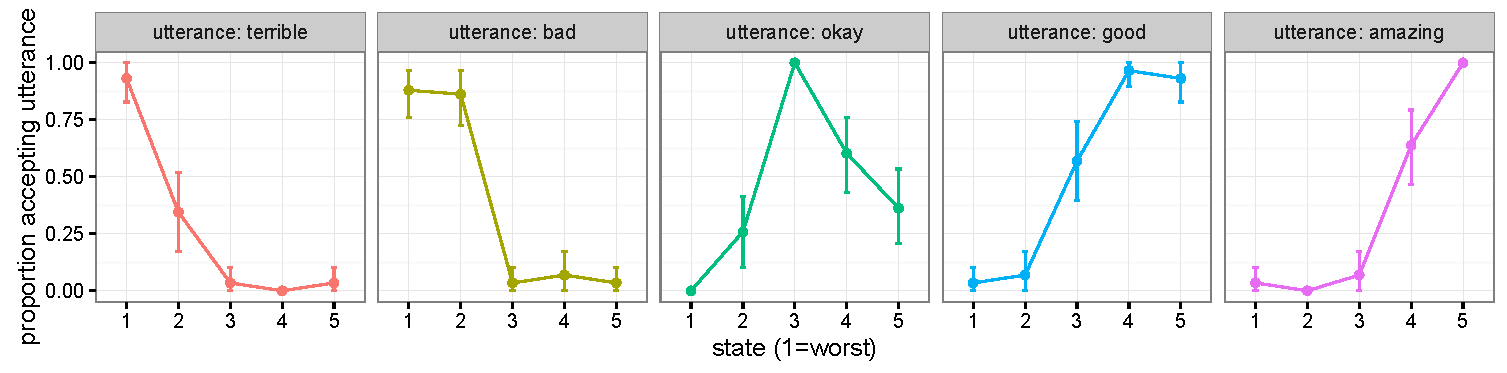
\includegraphics[width=.9\textwidth]{figures/exp1.pdf}
  \caption{\label{fig:exp1} Results from Experiment 1. Proportion of acceptances of words (shown in different colors) given the true state represented on a scale of hearts. Error bars represent 95\% confidence intervals.}
  \end{center} 
\end{figure*}

\subsection{Experiment 2: Goal inference}

Experiment 1 results were used as prior expectations for state-utterance mapping to generate the model of utterance production (speaker) and interpretation (pragmatic listener). Experiments 2 and 3 probed people's derivation of the speaker's goals and the true state, to be compared against predictions of our model. 

\subsubsection{Method} 

We presented scenarios in which a person (e.g., Ann) gave some performance and asked for another person (e.g., Bob)'s opinion on the performance. The same context items and true states as Experiment 1 were used. Additionally, we provided information on what Bob actually said to Ann (e.g., ``Your cake was okay''), where Bob used one of the five possible words,  \emph{terrible}, \emph{bad}, \emph{okay}, \emph{good}, and \emph{amazing}. Then we asked participants to infer the likelihood of Bob's goals to be honest, nice, and mean: the question read, ``Based on what Bob said, how likely do you think that Bob's goal was to be: honest; nice; mean,'' with the three goals placed in a random order below three slider bars, on which the participant could indicate each goal's likelihood.

\begin{figure*}[t]
\begin{center} 
  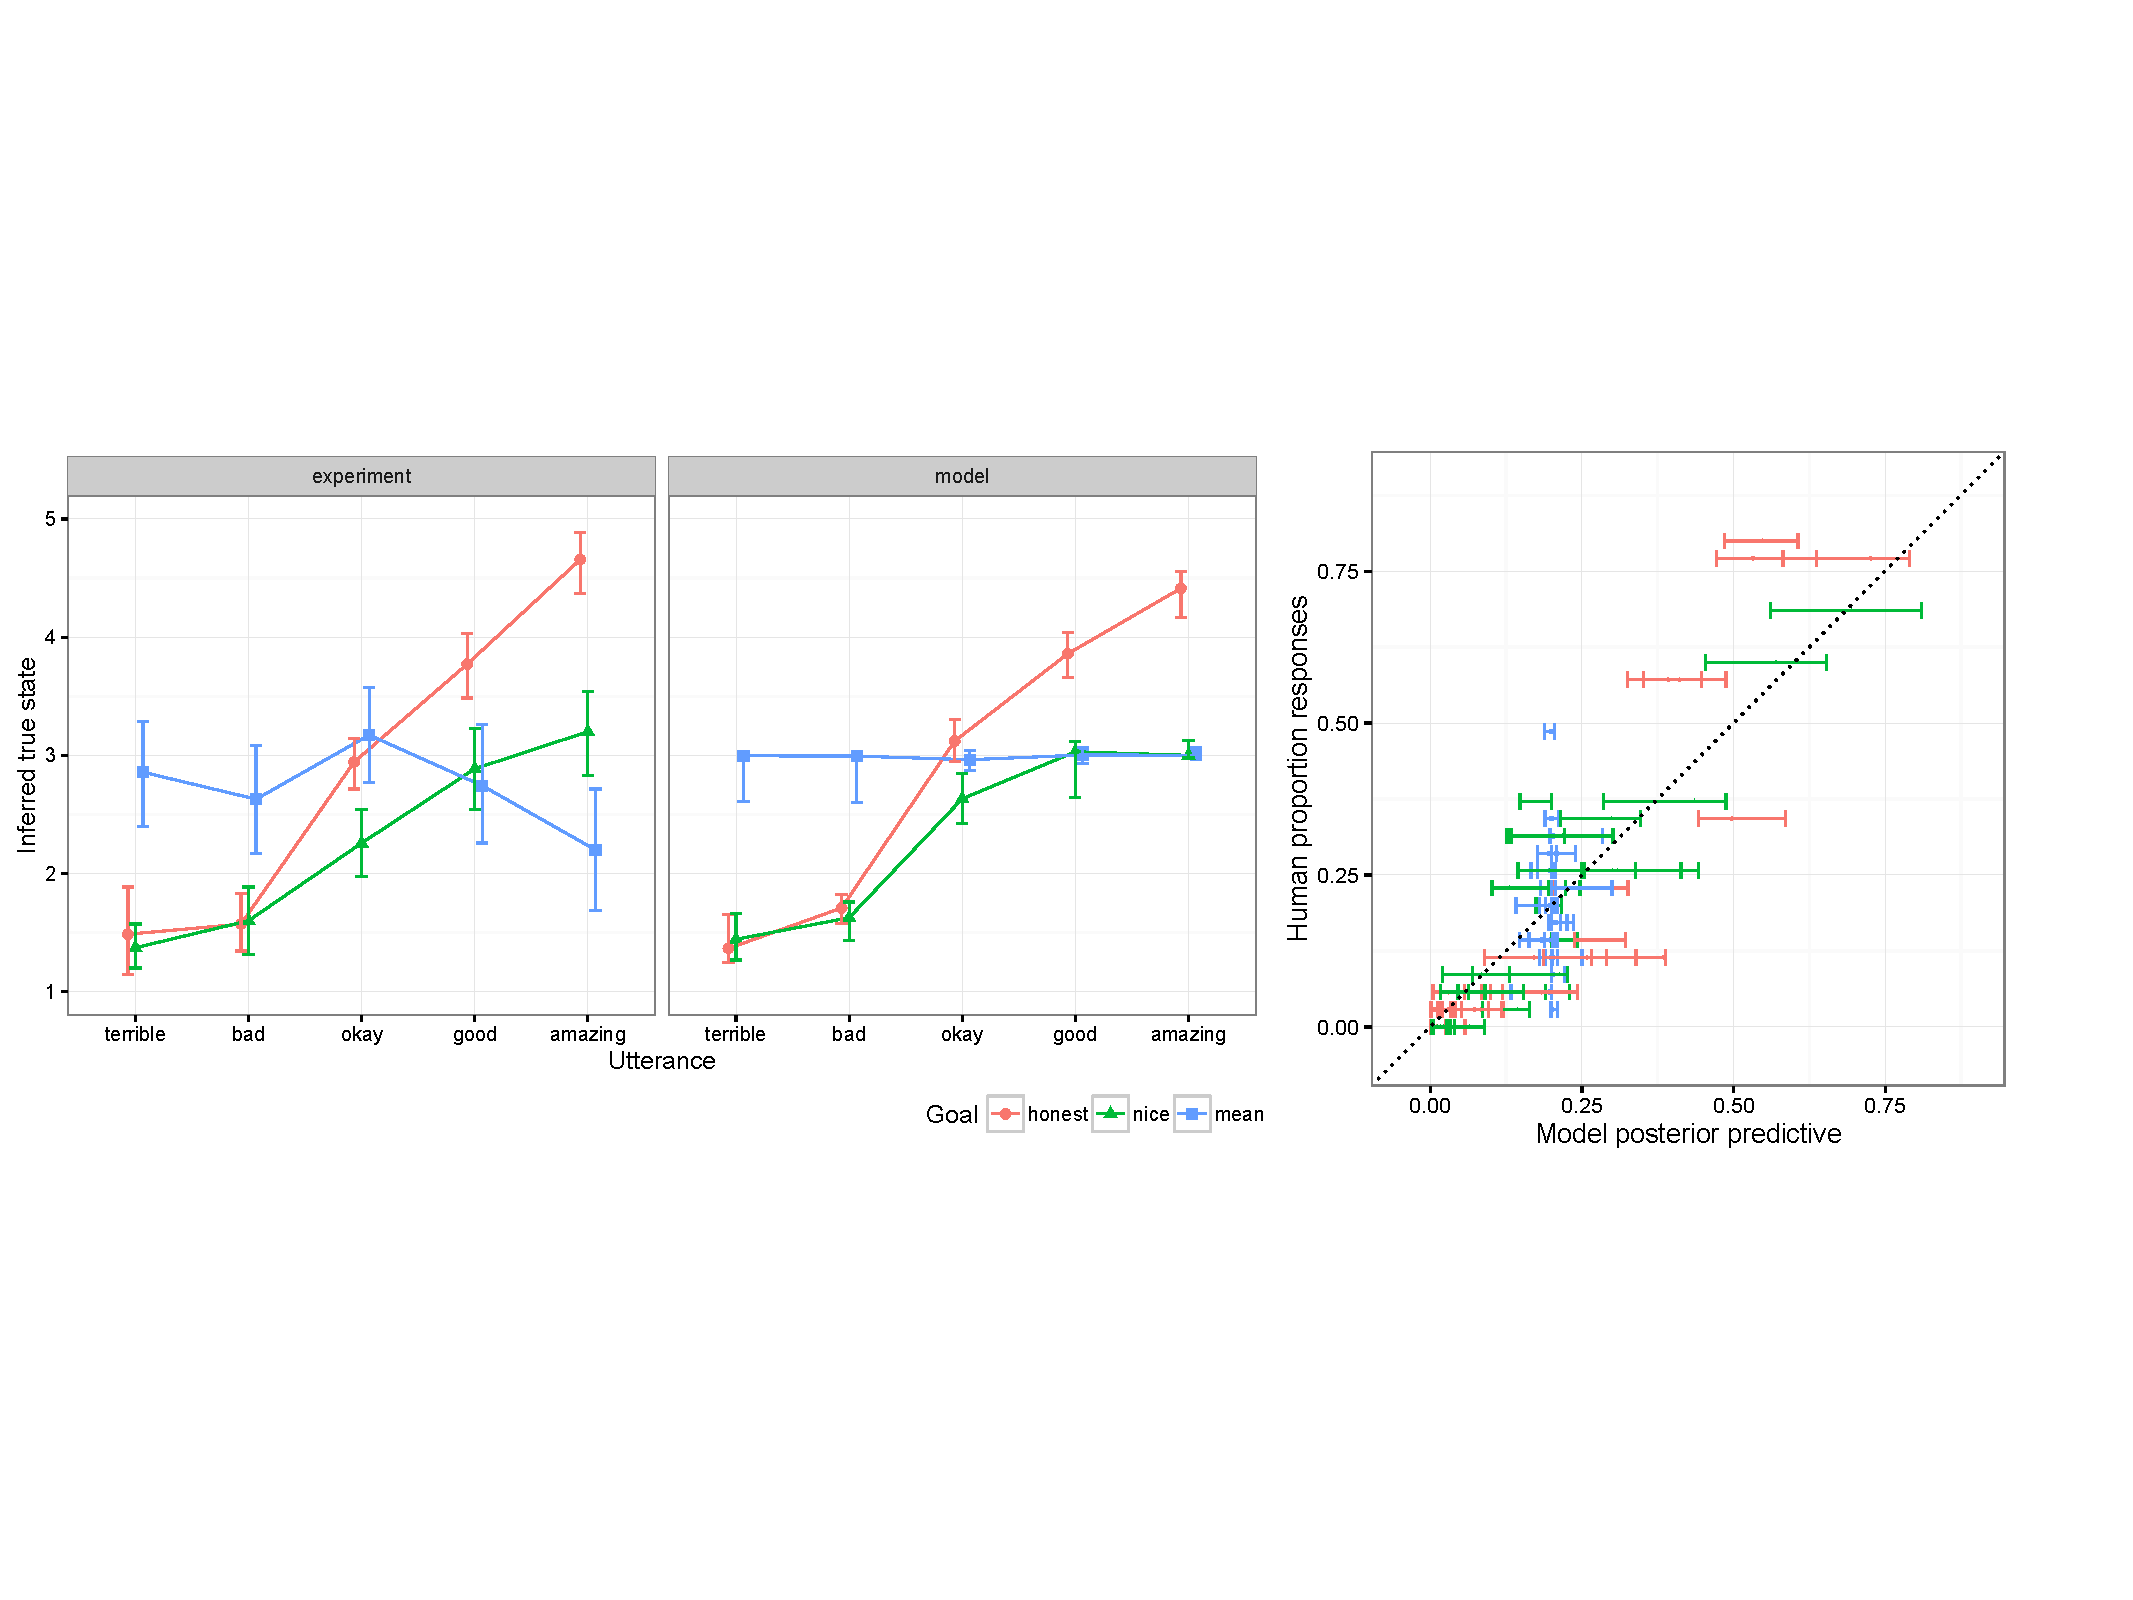
\includegraphics[width=.9\textwidth]{figures/exp2.pdf}
  \caption{\label{fig:exp2} Results from Experiment 2 (top) and model predictions (bottom). Attribution of speaker's goals (honest vs. nice vs. mean, shown in different colors) based on the true state and utterance. Error bars represent 95\% confidence intervals.}
  \end{center} 
\end{figure*}

\subsubsection{Results}

\begin{table}[t]
\caption{\label{tab:lmer1}  Coefficient estimates from mixed-effects models predicting goal attributions in Experiment 2.} 
\begin{center} 
\begin{tabular}{l r r r l} 
\hline
Predictor  &  Value (SE) & \emph{t}-value\\
\hline
\emph{Goal to be honest} \\
Intercept  & 1.5 (.04) & 34.1 \\
True state & -.35 (.01) &  -29.9 \\
Utterance & -.32 (.01) & -26.6 \\
True state $\times$ Utterance & .11 (.003) & 31.9 \\
\emph{Goal to be nice} \\
Intercept  & .07 (.04) & 1.70\\
True state & -.05 (.01) &  -5.46 \\
Utterance & .17 (.01) & 12.7 \\
True state $\times$ Utterance & .01 (.002) & 2.73 \\
\emph{Goal to be mean} \\ 
Intercept  & .37 (.04) & 9.18 \\
True state & .18 (.01) &  18.3 \\
Utterance & -.05 (.01) & -3.76 \\
True state $\times$ Utterance & -.04 (.003) & -12.2 \\
\hline
\end{tabular} 
\end{center} 
\end{table}

Participants attributed likelihoods for speaker's goals differentially depending on the true state and utterance. We fit linear mixed-effects models to measure the effects of true state and utterance (as numeric variables, ordered from the worst to the best) on the attribution of each goal (Table \ref{tab:lmer1}) and we found significant main effects and interactions of true state and utterance on each of all three goal attributions, though with varying effect sizes. Below we lay out some primary patterns shown in the data. % model: goal_prob ~ true_state * utterance + (utterance | subid)

Participants' attribution of goal to be honest (``honesty goal'') varied depending on the combination of state and utterance, as evidenced by the high effect size of the interaction. The peak in the likelihood of honesty goal attribution occurred when the literal meaning of the utterance was close to the true state, based on the literal semantics distribution shown in Experiment 1. The honesty goal attribution was highly correlated with the literal semantics distribution given the state and utterance (r = 0.86).

Attribution of goal to be nice (``niceness goal'') generally showed slightly decreasing slope with improved true state given particular utterance (represented by each facet in Figure \ref{fig:exp2}). For example, the utterance ``okay'' was associated with higher likelihood for niceness goal given negative true states of 1 and 2, but with lower likelihood given positive states of 4 and 5. This perhaps reflects people's reasoning that an utterance is ``nice'' if its literal meaning is more positive than the actual state. Attribution of goal to be mean (``meanness goal'') showed an opposite pattern to the niceness goal attribution: its slope across different utterances generally increased as true state improved, indicating that un utterance is perceived to be mean when the literal meaning is more negative than the actual state.

There was an interesting asymmetry between the niceness versus meanness goal attribution, in that positive utterances were associated with niceness goal regardless of the state, whereas negative utterances were only perceived to be mean given a positive (thus mismatching) true state. For example the utterance ``amazing'' is linked to the niceness goal with high likelihoods across all states; the utterance ``terrible'' is linked to meanness goal only for positive states but not negative states (the attribution is only at chance level of 50\% for state of 1). This perhaps reflects participants' lay notion of an optimal speaker who tries to be kind and honest; speaker's critical remark (e.g., ``bad'') is perceived to be out of a good will to be maximally truthful to the listener, rather than intention to damage the listener's reputation.

\subsection{Experiment 3: State inference}

\subsubsection{Method}

The procedure was the same as Experiment 2, except that, instead of providing information on the speaker (e.g., Bob)'s utterance and feelings about a person (e.g., Ann)'s performance (\emph{true state}) and asking for inference on Bob's goals, we provided information on Bob's utterance and his \emph{goal} (e.g., the prompt read: ``Bob wanted to be nice: ``It was okay,'' he said''), and asked for participants' inference on the true state (i.e., Bob's true feelings about Ann's performance), which they indicated on a scale of five hearts.

\subsubsection{Results}

\begin{table}[t]
\caption{\label{tab:lmer2}  Coefficient estimates from a mixed-effects model predicting state inferences in Experiment 3.} 
\begin{center} 
\begin{tabular}{l r r r l} 
\hline
Predictor  &  Value (SE) & \emph{t}-value\\
\hline
Intercept (Honesty goal)  & 1.4 (.16) & 8.91 \\
Utterance & .41 (.05) &  8.58 \\
Niceness goal  & 1.9 (.19) & 10.2 \\
Meanness goal & .75 (.19) & 4.03 \\
Utterance $\times$ Niceness goal & -.69 (.05) & -13.5 \\
Utterance $\times$ Meanness goal & -.11 (.05) & -2.15 \\
\hline
\end{tabular} 
\end{center} 
\end{table}

Inference of the actual rating for listener's performance, or the true state, varied depending on speaker's goal and utterance (Figure \ref{fig:exp3}). We fit a linear mixed-effects model to look at the effects of information on speaker's goal and utterance on inferred true states, and found significant main effects for and interactions between utterance and goal. Below we describe main patterns in the data.

Given the speaker's goal to be honest, as predicted from the literal semantics distribution, inferred state positivity was correlated with utterance positivity: ``terrible'' implied approximately the true state of 1, ``okay'' the state of 3, ``amazing'' the state of 5. Interestingly, state inferred based on the utterance ``[It was] bad'' was not judged to be different from the inferred state based on ``terrible,'' which is seemingly more negatively-connoted. In contrast, the inferred state based on ``good'' was less positive than inferred based on ``amazing.'' This may suggest that saying even a weakly negative remark (e.g., ``bad'') is face-threatening to a similar degree as making a more strongly negative comment, given that the speaker has already decided to express criticism.

Given the speaker's goal to be nice, the inferred state positivity also increased with the utterance positivity, but participants inferred that the states are less positive compared to states given honesty goal, based on neutral and positive utterances. Based on the utterance ``amazing,'' participants inferred the true state to be close to 5 given the honesty goal, but they inferred the state to be around 3 given the niceness goal. This suggests that participants thought a speaker who was trying to be nice produced an utterance  with a literal meaning that is more positive that the speaker's true feelings toward the listener's performance.

It should be noted that more positive utterances lead to inference of more positive states given the goal to be nice, which indicates that people think a ``nice'' speaker is still being somewhat informative with respect to communicating what the true state is. Thus, a nice speaker probably used the word ``amazing'' to describe an okay presentation rather than a terrible one.

Curiously, inferred states based on honesty and niceness goals did not differ from each other given negative utterances (``terrible'' and ``bad''). Thus, given a speaker who tried to be nice and said ``bad,'' participants did not infer the true state to be worse than the state inferred given a speaker who tried to be honest and said ``bad.'' This may indicate a link between the two utilities we posited: ``bad'' is a negative utterance, which suggests it was impossible for the speaker to be ``nice'' and satisfy the social utility, to save the listener's face. But a speaker who tried to cooperate with the listener by being nice would also want to cooperate in another sense, by being honest and satisfying the epistemic utility.  Thus, participants might have reasoned that the speaker encountered an impossible situation to be cooperative with niceness and instead decided to cooperate with honesty. 

Finally, given the speaker's goal to be mean, participants inferred that the true states were more positive if the speaker's utterance was negative or neutral. Thus, they judged that a mean speaker saying ``terrible'' meant it was not terrible but okay (state of 3). Interestingly, if a positive utterance was produced with the goal to be mean, the true state was inferred to be worse compared to the states based on honesty and niceness goal. That is, a mean speaker saying ``amazing'' was judged to mean that the state was worse than average. This may be due to irony in play: making an extremely positive remark about an extremely bad performance is perceived to be sarcastic and ill-intentioned \cite{colston1997}. Our current model does not include a component of sarcasm, and it will be an interesting and useful addition in the future.

\begin{figure}
\begin{centering} 
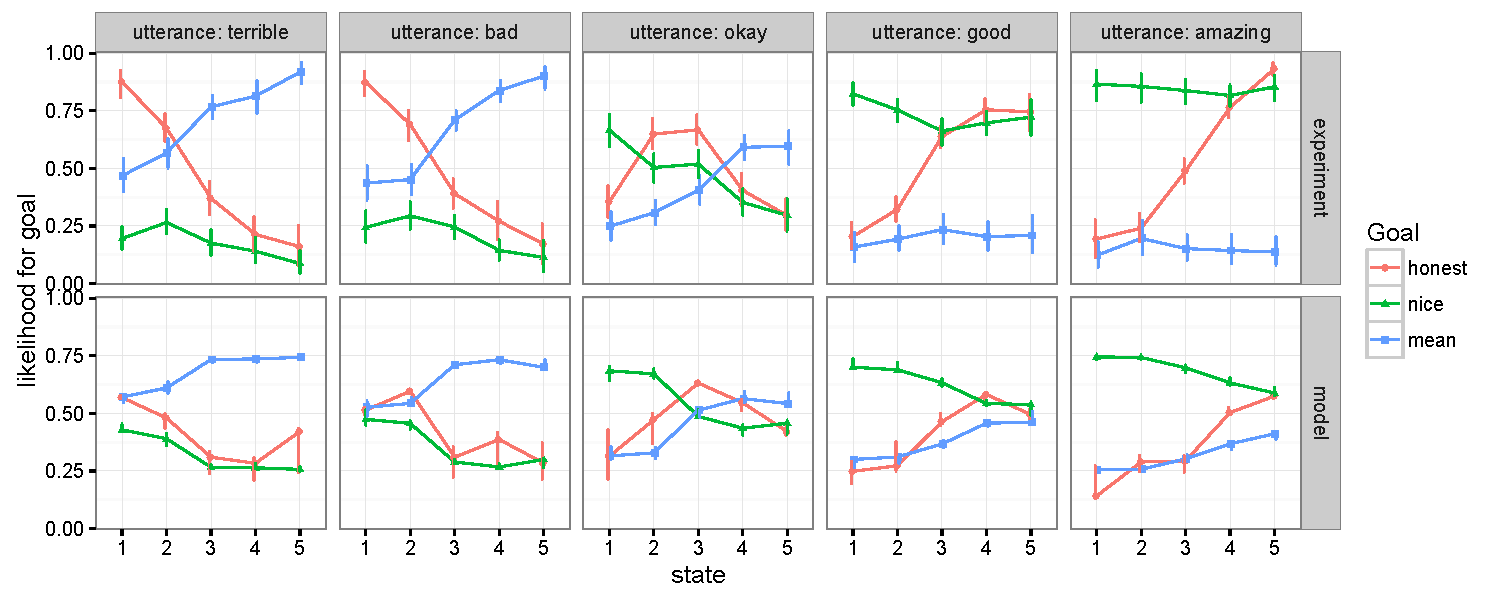
\includegraphics[width=3.2in]{figures/exp3.pdf}
\caption{\label{fig:exp3} Results from Experiment 3. Average states inferred based on speaker's goal and utterance. Error bars represent 95\% confidence intervals.}
\end{centering} 
\end{figure}

\section{Model behavior}

We now turn to the predictions of the computational model.
The model in Eq.~\ref{eq:L1} specifies a joint-belief distribution over the speaker's goals $\beta$ and possible states of the world $s$.
We compare these predictions to the experimental data from Expt.~2 \& 3, respectively.

\subsection{Model details and priors}

We use the experimental data from Expt.~1 as the literal meaning of utterances $W$ with respect to states $S$ --- \denote{w}(s).
We assume a uniform prior distribution over possible states of the world $s\sim \text{DiscreteUniform} \{1, 2, 3, 4, 5\}$. 

For ease of comparison to the experimental data, we separate $\beta_{social}$ into a positive component ($\beta_{nice}$) and a negative component ($\beta_{mean}$), writing the utility function now as
$$
U(w;s; \beta) = \beta_{e}\cdot U_{epistemic} + (\beta_{nice} - \beta_{mean}) \cdot U_{social}
$$

In addition, in each model, we include an explicit submodel of random guessing behavior, and model the behavioral data as mixture of this noise and the predictions of the pragmatic listener model $L_1$ (Eq.~\ref{eq:L1}).
Including such a contamination parameter is important for getting reliable estimates of the parameters of the RSA model, which would otherwise be corrupted by this noise \cite{LW2014}. 
We put a uniform prior over this mixture parameter $\phi \sim \text{Uniform}(0,1)$. 
This mixture parameter provides an additional measure of goodness of fit: It shows the proportion of the data that is better explained by the cognitive model than by a model of random guessing. 

\subsection{Goal inference}

In Experiment 2, participants were supplied with the ``true state'' $s$ as well as the speaker's utterance $w$, and were asked to rate the likely goals of the speaker. 
Here, we assume a uniform prior over the likely goals of the speaker, which is operationalized in the computational model as weights over the utilities: $\beta \sim \text{Uniform}(0,1)$ .


The computational model then has 2 parameters: the speaker optimality parameter $\lambda$ in Eq.~\ref{eq:S1} and the value scale parameter $\alpha$ in the utility function. 
We put uninformative priors on these and infer their credible values using Bayesian inference.
\begin{eqnarray*}
& \lambda \sim \text{Uniform}(0,20)\\
& \alpha \sim \text{Uniform}(0, 5)
\end{eqnarray*}
We ran 3 MCMC chains for 40,000 iterations, discarding the first 20,000 for burnin.
The Maximum A-Posteriori (MAP) estimate and 95\% Highest Probability Density Interval (HDI) for $\lambda$ is 6.8 [5.7, 7.8]; for $\alpha$ is 1.03 [0.91, 1.19]; for $\phi$ is 0.09 [0.06, 0.13].
This is a relatively low value for $\phi$: The model explains about 90\% of the data set better than a model of random guessing.

%               Goal Parameter        MAP    credLow  credHigh
%             (fctr)    (fctr)      (dbl)      (dbl)     (dbl)
%1             alpha        NA 1.02553704 0.91319156 1.1865188
%2               phi        NA 0.08983868 0.05699245 0.1284084
%3 speakerOptimality        NA 6.81149016 5.76426562 7.8453595

To test what data the model actually predicts, we examine the posterior predictive distribution by marginalizing out the likely parameter values and generating predictions for what the data should look like, given our cognitive model and the inferred parameters.
The predictions of the model are shown in Figure \ref{fig:exp2}.
\mht{Describe model predictions.}
Overall, the model explains a lot of the variance in the goal inference data $r^2(75) = 0.87$.

\subsection{State inference}

In Experiment 3, participants were told what the speaker said $w$ as well as described what the speakers intentions were (e.g. \emph{Bob wanted to be nice}). 
To model this, we assume that the intentions (e.g. \emph{wanted to be nice}) modified the listener's prior distribution over goal-weights for the relevant goal. For example, if a speaker was trying to be nice, we interpret that to mean the speaker has a non-uniform prior distribution over $\beta_{nice}$ (in particular, $\beta_{nice}$ should be skewed toward higher-values). 
We assume $\beta \sim \text{Beta}(\gamma, \delta)$, and for each goal condition (trying to be \emph{nice, mean, honest}), we put uninformative hyperpriors over the associated goal prior\footnote{For ease of interpretation, we are parametrizing the $\beta$ distribution by its mean and concentration. To recover the canonical shape parametrization, use $\gamma \delta$ and $(1-\gamma)\delta$.}.
For the unassociated goal priors (e.g. $\beta_{mean}$ and $\beta_{honest}$ when \emph{trying to be nice}), we use the same uniform priors we used to model the goal inference data.
%
\begin{eqnarray*}
& \gamma \sim  \text{Uniform}(0,1)\\
& \delta  \sim  \text{Uniform}(0, 20)
\end{eqnarray*}

\begin{table}[]
\centering
\label{my-table}
\begin{tabular}{lll}
\hline
Experimental Condition (Goal) & Mean & Concentration \\ \hline
(trying to be) Honest                        &      &               \\
(trying to be) Nice                          &      &               \\
(trying to be) Mean                          &      &               \\ \hline
\end{tabular}
\caption{Inferred hyper-parameter values for Goal Priors in State Inference task.
For each experimental condition (trying to be X), we inferred the likely priors on the goal weights for the associated goal.
Values shown are MAP estimates and 95\% HDI for the parameter values.}
\end{table}
We ran 3 MCMC chains for 20,000 iterations, discarding the first 10,000 for burnin.
The MAP and 95\% HDI for $\lambda$ is \red{6.8 [5.7, 7.8]}; for $\alpha$ is \red{1.03 [0.91, 1.19]}; for $\phi$ is \red{0.09 [0.06, 0.13]}.
Inferred parameter values for the goal priors are shown in Table 1.

The predictions of the model are shown in Figure \ref{fig:exp3}.
\mht{Describe model predictions.}
\mht{Model-data correlation}. 

\section{Discussion}

% politeness as integration of two kinds of goals in an informing context: improving the listener's epistemic state, and face-saving
% information transfer is not the only goal speaker has; the social function of making the listener feel good, and thereby establishing a favorable social relationship is another important goal of conversation.
% our computational model that represents both types of utilities (epistemic and social) successfully capture key patterns in the empirical data

% next step: 
% interaction with implicatures
% politeness at what level? - is the polite utterance meant to be a lie (thus the listener is misinformed) or an indirect expression (thus the listener reaches a full epistemic state), and this depends on what?

\bibliographystyle{apacite}

\setlength{\bibleftmargin}{.125in}
\setlength{\bibindent}{-\bibleftmargin}

\bibliography{politeness}


\end{document}
